\documentclass{article}
\usepackage{amsmath}
\usepackage[T1]{fontenc}
\usepackage[table]{xcolor}
\usepackage{minted}
\usepackage{enumitem}
\usepackage{siunitx}
\usepackage{booktabs}
\usepackage{graphicx}
\usepackage{float}
\usepackage[margin=1in]{geometry}
\usepackage{url}

\newtheorem{lemma}{Lemma}[section]
\newenvironment{proof}{\par\noindent\textbf{Proof of Lemma \thelemma.}\ \itshape}{\par}

\title{On the Correctness of Ukkonen's Algorithm Without Suffix Links\\[0.5em] \large A Practical Commentary on Suffix Tree Construction\\ \small Advanced Algorithms Assignment 1}
\author{Nicholas.S}
\date{\today}


\begin{document}
	\maketitle
	\begin{abstract}
		In this document, a naive implementation for Ukkonen's algorithm without suffix links has a worst case running time of $O(n^2)$ for suffix tree construction.  The algorithm follows three extension rules, and must traverse down edges individually to create a split.  It becomes evident, through a step-by-step visualised walk-through, that the suffix link implementation is far better optimised, running in linear time relative to the size of the input string.  Additionally, the implementation code is provided with an in-depth correctness commentary on how each step contributes to running each extension rule, necessary pre and post-conditions, effect on the loop invariant and the importance of each step.
	\end{abstract}
	\noindent\textbf{Keywords: } Ukkonen's algorithm, suffix trees, suffix links, correctness commentary, string, lemma, proof
	
	\newpage
	\tableofcontents
	\newpage
	
	\section{Introduction}
	Ukkonen's algorithm is uniquely known for constructing a suffix tree where the input string is read from left-to-right.  It was formalised by Esko Ukkonen in ``On-line construction of suffix trees'' \cite{ukkonen1995}, and at any step of the construction, there is a valid implicit suffix tree. Suffix trees were introduced in ``Linear Pattern Matching Algorithms'' \cite{weiner1973}, as a way to reduce basic string operations in reduced time from standard algorithms. \\
	My own implementation of Ukkonen's is a naive approach, where each edge is traversed manually from the root on each iteration, whenever the edge is reset.  Whilst it still returns a valid and fully constructed suffix tree of any string which doesn't contain the character '\$', the worst case upper bound is $O(n^2)$ where n is the length of the string. The main advantage of my implementation, however, is that there is some form of reduced space consumption because there is no stored suffix link.
	
	\subsection{The Three Rules of Ukkonen's}
	To understand Ukkonen's algorithm, there are three essential rules to how it exactly works.  Let there exist string $s$ such that $s = s_0, s_1 \dots s_n$.  Then, assume we have already some online, partially constructed suffix tree of $s$, denoted as $T$.  Then, let us use $i$ and $j$ as indices such that $0 \le i \le j \le n + 1$, where $j + 1$ represents the current character being processed.
	\begin{enumerate}[label=(Rule.\arabic*)]
		\item  If the path from $s[i\dots j]$ ends on a leaf edge, then $s[j + 1]$ is inserted such that the path is now $s[i\dots j+ 1]$ \cite[p.~9, l.~6]{gomez}.
		\item  If the path from $s[i\dots j]$ ends on a non-leaf edge, where $0 \le k \le j$, then remain on the edge until some $j + k$, such that $s[i\dots j] != j + k]$.  At this point, split the existing edge from $(i\dots i + k)$, with two child nodes containing edges $(j + k, j + k)$, and $(i + k, j + k)$ \cite[p.~9, l.~7]{gomez}.
		\item  Otherwise, $s[i + k]$ moves on without insertion \cite[p.~9, l.~8]{gomez}.
	\end{enumerate}
	
	\clearpage
	\section{Code Implementation in C++}
	\subsection{Brief Explanation}
	The following code was my own hand-written implementation of the naive Ukkonen's without suffix links.  The code contains a header file with the necessary structs to implement the algorithm.  This file is imported into the source file, which implements the \textit{create} function to return the root node of a constructed suffix tree based on the given word.  \\
	There is no ability to search, the only example of it running is against JSON test cases with my own implementation of the test runner.
	\\
	It's quite clear that the code does not represent the initial pseudocode provided in 'online construction' page 12.  This was an intentional move to try to derive the code through only a theoretical understanding.

	\subsection{Header File}
	\inputminted[linenos, frame=lines, fontsize=\scriptsize, tabsize=4, breaklines, label={src/headers/suffix\_tree.hpp}]{cpp}{../src/headers/suffix_tree.hpp}

	\subsection{Source File}
	\inputminted[linenos, frame=lines, fontsize=\scriptsize, tabsize=4, breaklines, label={src/suffix\_tree.cpp}]{cpp}{../src/suffix_tree.cpp}
	
	\clearpage
	\section{A Worked Example}
	
	\subsection{Algorithm Walk-through}
	The following is a visualised, step-by-step walk-through of how my implementation constructs 'aabab' into a suffix tree. 
	\paragraph{Active Point (A), \textit{lines 29:38, header}.}  A struct which contains pointers to nodes \textit{parent} and \textit{edge}, and an integer \textit{length}.  The \textit{parent}, $\rho$, is a node which is being searched for an edge, this is used to confirm if a character already exists at this point in the tree.  The \textit{edge}, $e$ is a pointer to a node such that $(a, b)$ form the indices of an edge to $\rho$, $s[a\dots b]$.  The \textit{length}, $len$, variable is used to label how far into $e$ is being processed.  For example, $ len = 2$ means the comparison is with some $s[a + len]$.
	
	\paragraph{Remainder (R), \textit{line 27, source}.}  An integer which denotes the number of suffixes which have been skipped.  This is being applied, where the suffixes will eventually be implemented at a later time.
	
	\paragraph{Index (i), \textit{line 30}, \textit{source}.} A shared pointer which points to how far into the string 'aabab' the algorithm is up to.  For example, if \textbf{i} = 2, then up to 'aab' is being processed.  This is how extension rule one is applied in constant time.  Whenever some $e$ contains $(a, \textbf{i})$, then whenever \textbf{i} is altered, that same $e$ will instantly update to use the new value.  For example, if some node exists with $[0, i]$, then when $i = 0$, the node has indices $[0, 0]$.  When $i =1$, the indices will automatically become $[0, 1]$, that is how the shared pointer works.
	
	\paragraph{1. Initialisation, \textit{lines 14:30}.}
	\begin{figure}[H]
		\centering
		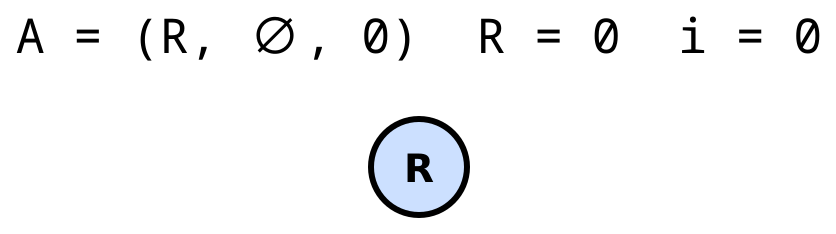
\includegraphics[scale=0.17]{media/Example/step00}
		\caption{The initial state, with only the root.}
		\label{fig:step00}
	\end{figure}
	The suffix tree root node \textbf{R} has been initialised, where the root has no incoming edge, and no children.  Also, $\rho =$ \textbf{R}.
	
	\paragraph{2. Create a New Node, \textit{lines 36:59}.}\leavevmode
	\begin{figure}[H]
		\centering
		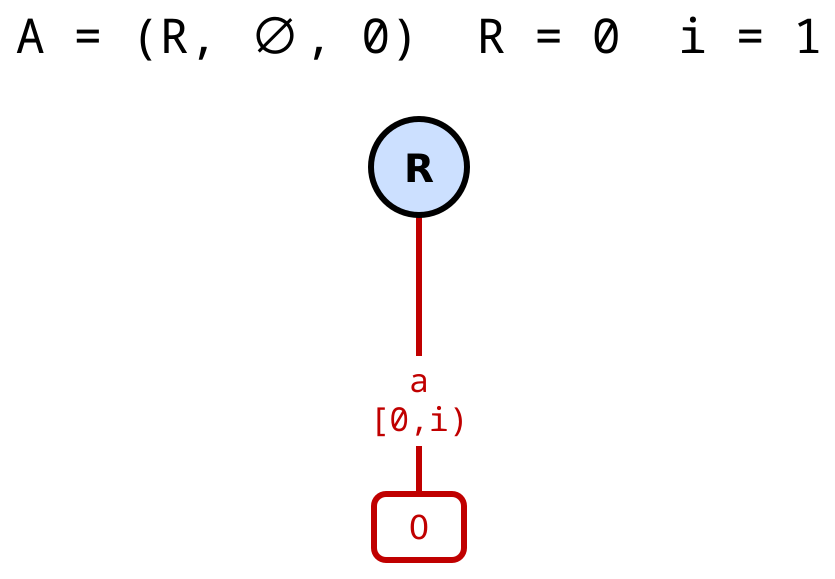
\includegraphics[scale=0.17]{media/Example/step01}
		\caption{A new leaf for \texttt{a} under the root.}
		\label{fig:step01}
	\end{figure}
	The loop begins.  $i$ begins as $0$, such that the word being processed is $s[0]$ which is 'a'.  Then, $\rho$ is searched to see whether it contains a child node that begins with 'a'.  Here, this is false, and so the new node is created from $[0, i]$.  This is a case of (Rule.2), where $\epsilon \ne$ 'a', and so the node is created.  Lastly, $i$ is increased by one, to mark the end of (Rule.2) so move to the next character.

	\paragraph{3. Skipping Operation, \textit{lines 113:122}.}\leavevmode
	\begin{figure}[H]
		\centering
		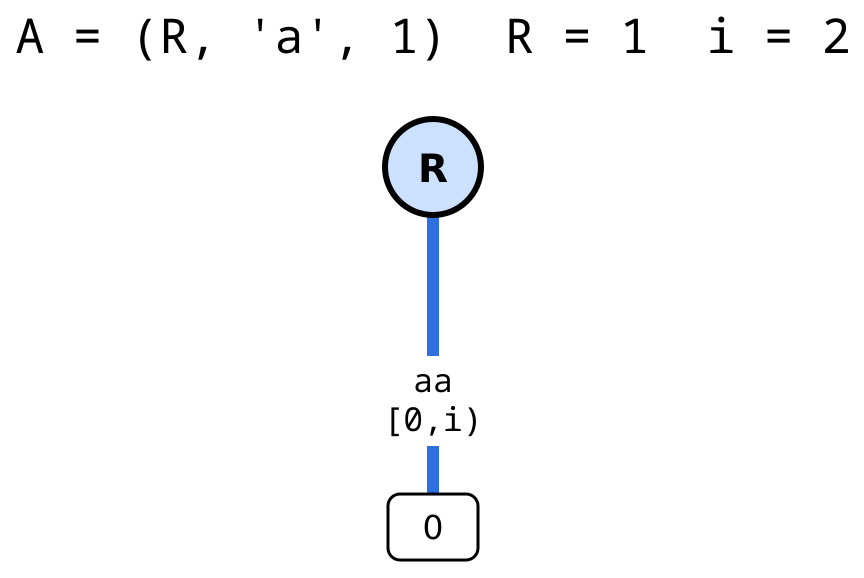
\includegraphics[scale=0.17]{media/Example/step02}
		\caption{Rule 3 defers the suffix \texttt{a}.}
		\label{fig:step02}
	\end{figure}
	At $i = 1$, $s[i] =$ 'a'.  Given $\rho$ contains a child node beginning with 'a', $e$ points to that node instead.  At this point, $len = 0$, and so this becomes $s[0] = s[1]$, where now (Rule.3) is applied, and nothing is done.  Then, $len = 1$ as the first characters have been compared, \textbf{R} = 1 to allow the current suffix to be inserted at a later time, and \textbf{i} = 2 .
	
	
	\paragraph{4. Split Current Edge and Create New Nodes, \textit{lines 76:110}.}\leavevmode
	\begin{figure}[H]
		\centering
		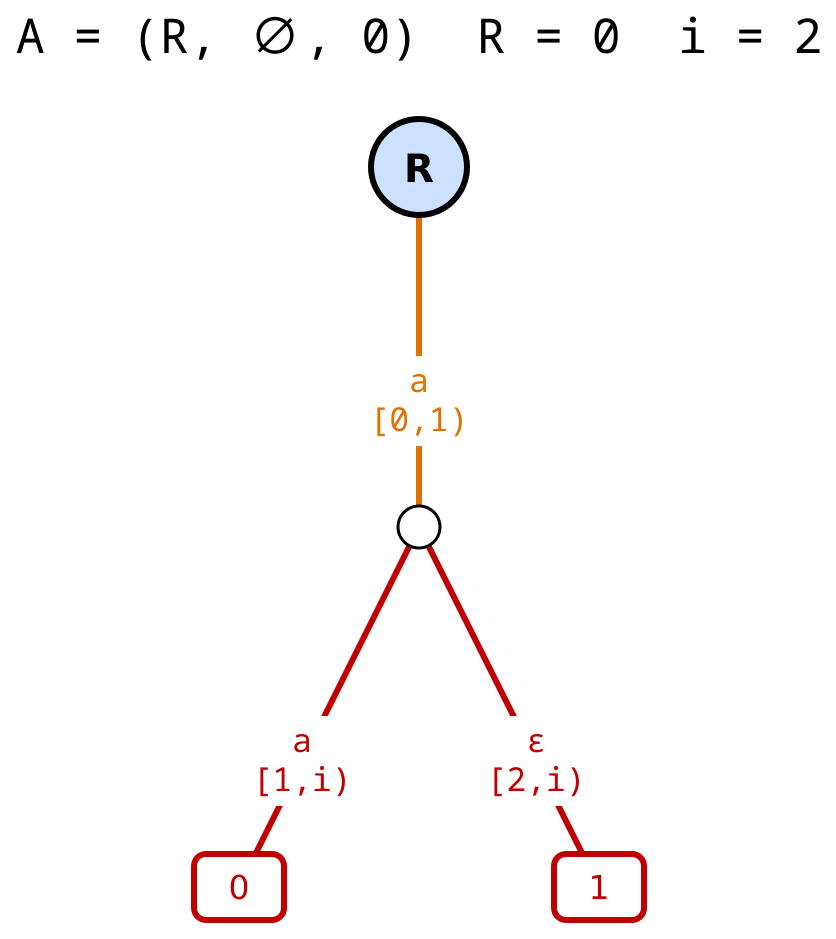
\includegraphics[scale=0.17]{media/Example/step03}
		\caption{The leaf \texttt{aa} is split after \texttt{a}.}
		\label{fig:step03}
	\end{figure}
	The only leaf edge in the tree node contains indices from (0, 2) now.  The current character, $s[\textbf{i}]$ is 'b'.  Because from path $s[0 + 1] = s[1]$, there exists $s[2]$ after such that $s[\textbf{i}] \ne s[\alpha + len]$, where $\alpha$ is the first index in $e$.  According to (Rule.2), the edge must now be split such that $e$ becomes (0, 1), then $e_0$ is created with (2, 2), and $e_1$ is created with (1, 2) as child nodes.  	

	\paragraph{5. Add New Node.}\leavevmode
	\begin{figure}[H]
		\centering
		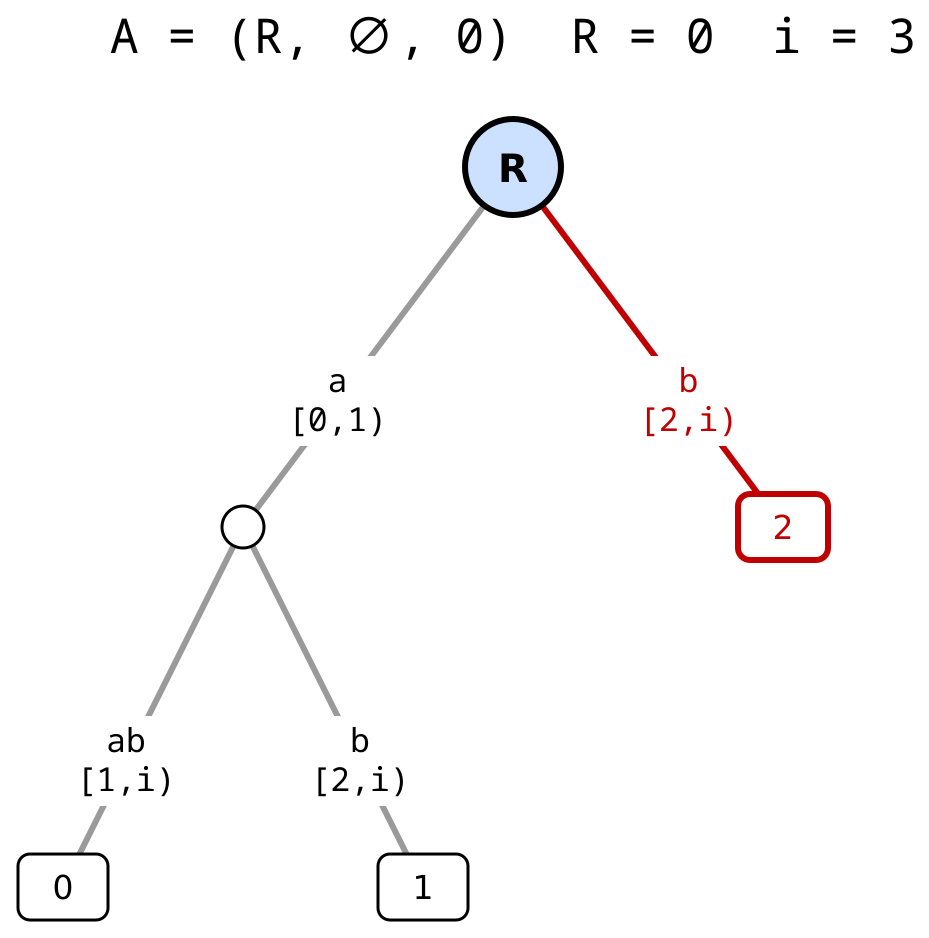
\includegraphics[scale=0.17]{media/Example/step04}
		\caption{A new leaf for \texttt{b} under the root.}
		\label{fig:step04}
	\end{figure}
	The split in the previous step inserted the suffix 'ab', so \textbf{R} = 0 and \textbf{i} stays at 2 to insert the final suffix 'b'.  With $len = 0$, $\rho$ is searched for a child beginning with $s[\textbf{i}] =$ 'b'.  None exists, so (Rule.2) creates a new node from $(2, \textbf{i})$.  Because \textbf{R} = 0, \textbf{i} is increased to 3.

	\paragraph{6. Search For Child Node.}\leavevmode
	\begin{figure}[H]
		\centering
		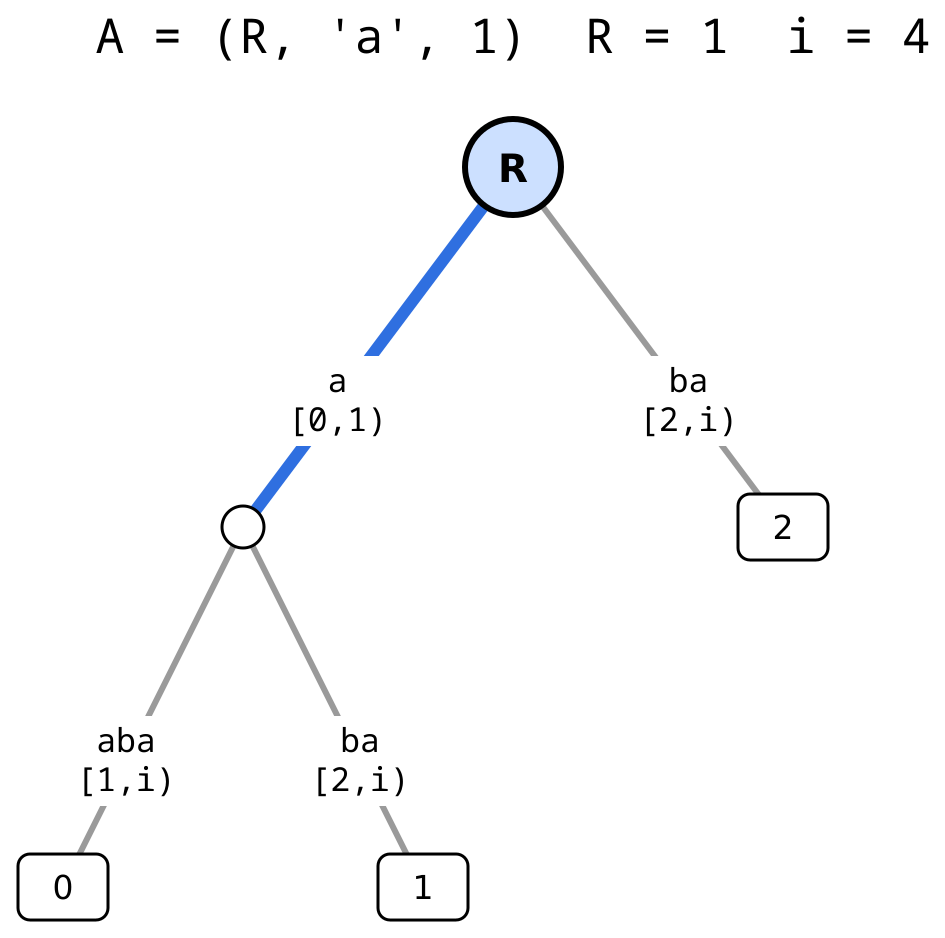
\includegraphics[scale=0.17]{media/Example/step05}
		\caption{Rule 3 defers the suffix \texttt{a} again.}
		\label{fig:step05}
	\end{figure}
	At \textbf{i} = 3, $s[\textbf{i}] =$ 'a'.  $\rho$ contains a child beginning with 'a', so $e$ points to the internal node with indices $(0, 1)$.  As $len = 0$, the comparison is $s[0] = s[3]$, which are both 'a', so (Rule.3) is applied and nothing is done.  Then $len = 1$, \textbf{R} = 1 and \textbf{i} = 4.
	
	\paragraph{7. Edge Traversal.}\leavevmode
	\begin{figure}[H]
		\centering
		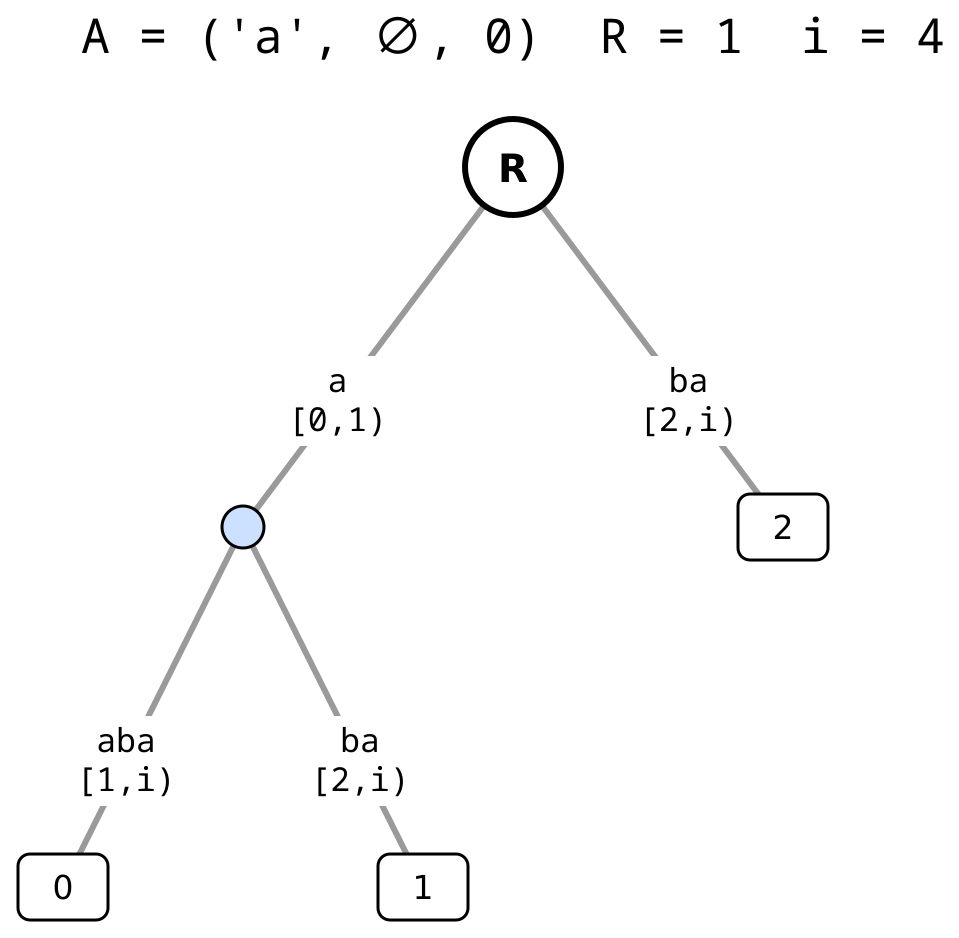
\includegraphics[scale=0.17]{media/Example/step06}
		\caption{The active point walks down to the internal node \texttt{a}.}
		\label{fig:step06}
	\end{figure}
	At \textbf{i} = 4, $e$ is chosen by $s[\textbf{i} - len] = s[3] =$ 'a', which is the internal node with indices $(0, 1)$.  Its edge has a length of 1, and $len = 1$ has reached its end, so there is no character left on $e$ to compare.  Lines 66:70 traverse down the edge: $\rho$ becomes the internal node, $len$ is reduced by the edge length to 0, and $e$ is cleared.  Nothing is inserted, so \textbf{R} and \textbf{i} are unchanged.

	\paragraph{8. Skipping Operation.}\leavevmode
	\begin{figure}[H]
		\centering
		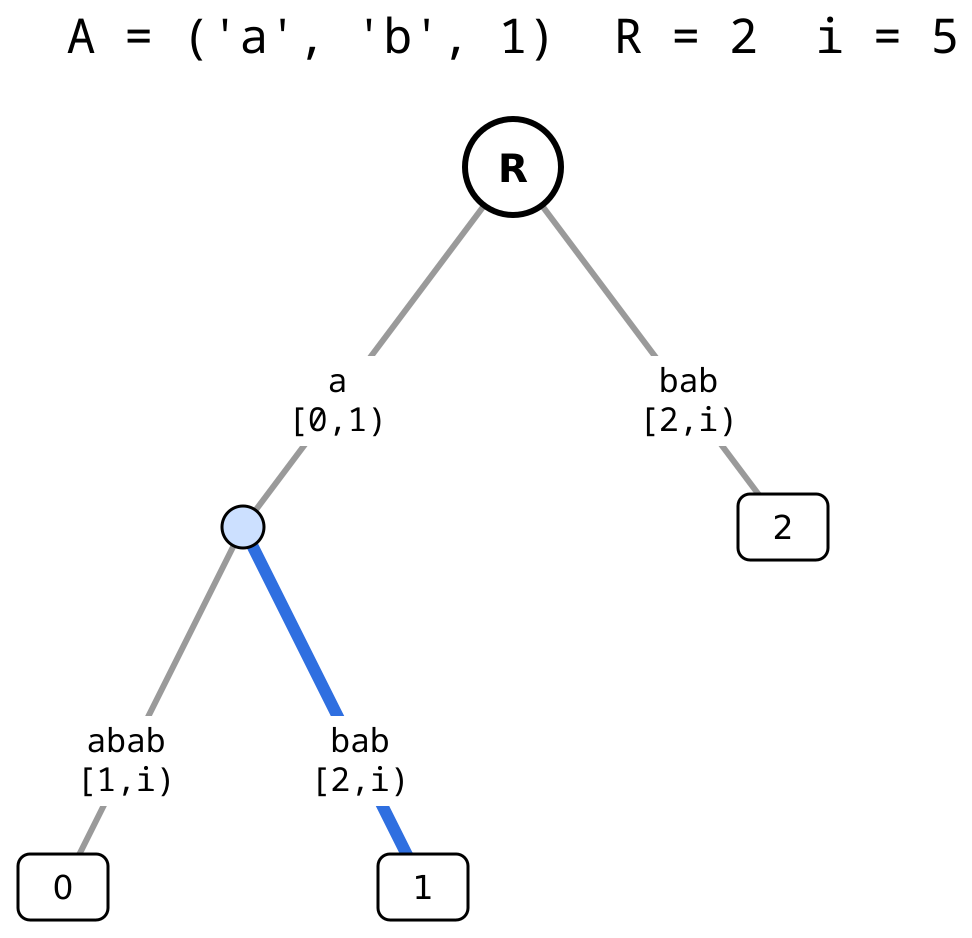
\includegraphics[scale=0.17]{media/Example/step07}
		\caption{Rule 3 below the internal node, with two suffixes pending.}
		\label{fig:step07}
	\end{figure}
	Still at \textbf{i} = 4, $\rho$ is now the internal node, and with $len = 0$ it is searched for a child beginning with $s[4] =$ 'b'.  That child is the leaf $(2, \textbf{i})$, and $s[2] = s[4] =$ 'b', so (Rule.3) applies again.  Then $len = 1$, \textbf{R} = 2 and \textbf{i} = 5, so two suffixes, 'ab' and 'b', are now waiting to be inserted.

	\paragraph{9. Split Current Edge.}\leavevmode
	\begin{figure}[H]
		\centering
		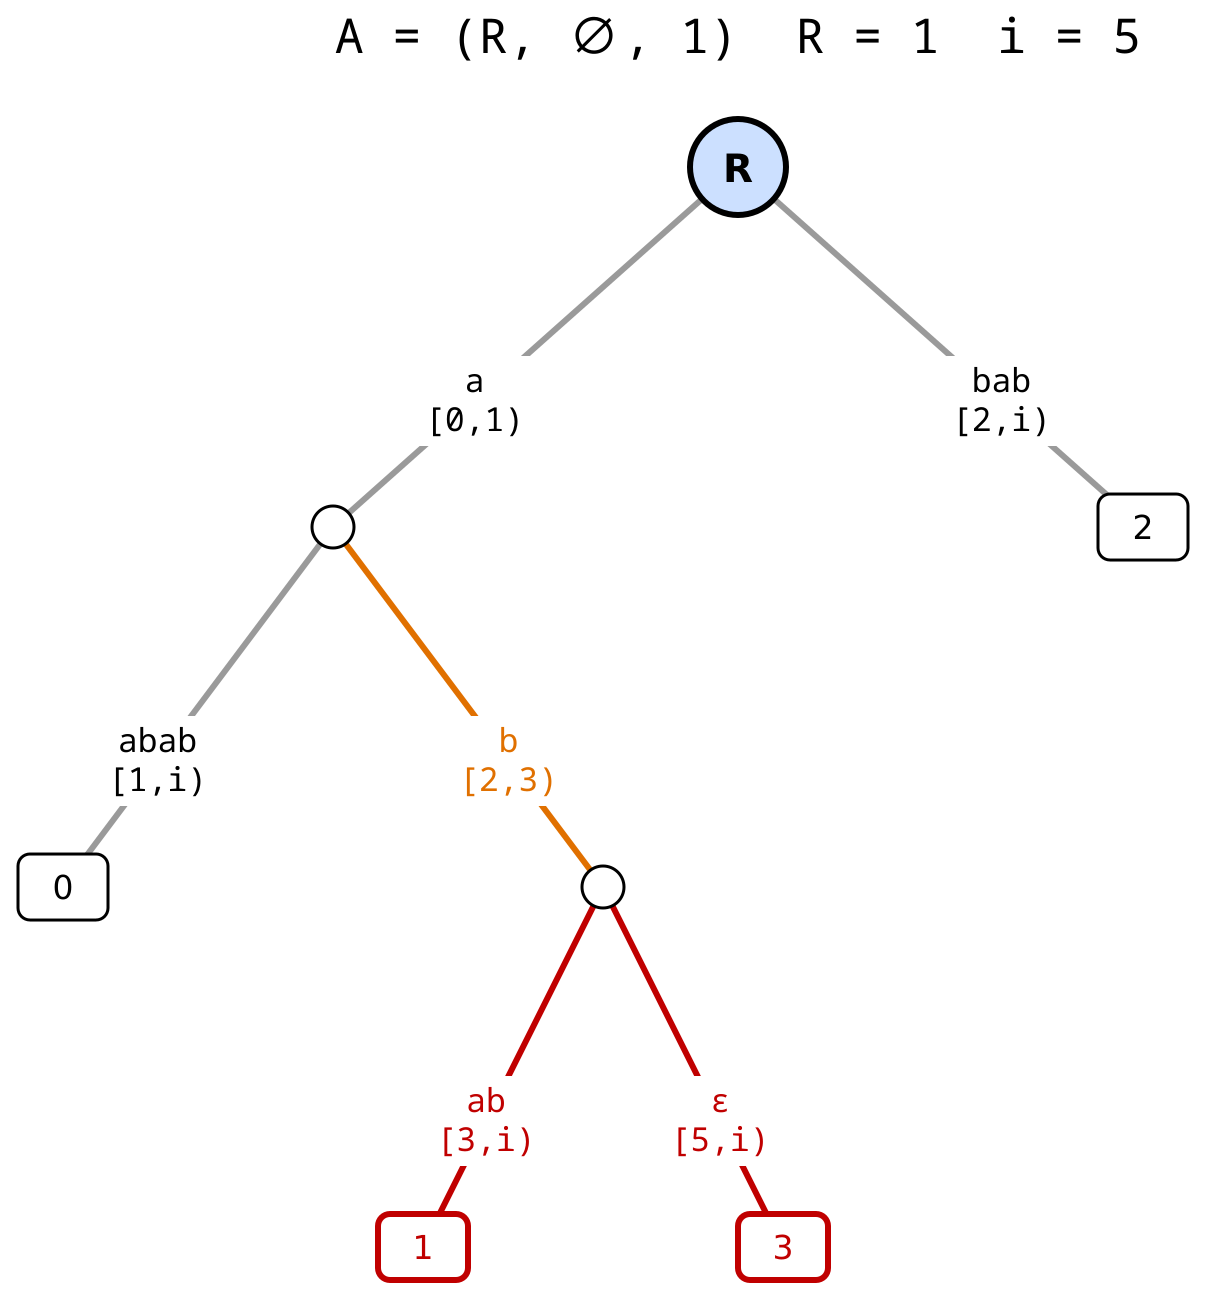
\includegraphics[scale=0.17]{media/Example/step08}
		\caption{The leaf \texttt{bab} below the internal node is split after \texttt{b}.}
		\label{fig:step08}
	\end{figure}
	At \textbf{i} = 5, the terminal character \$ is processed.  From the internal node, $e$ is the leaf $(2, \textbf{i})$, which spells 'bab'.  The next character on $e$ is $s[2 + len] = s[3] =$ 'a', which is not \$, so (Rule.2) splits $e$ into $(2, 3)$, with a new node $(5, \textbf{i})$ for \$ and a node $(3, \textbf{i})$ for the rest of the old edge.  This inserts the suffix 'ab\$'.  \textbf{R} is reduced to 1, so \textbf{i} stays at 5, and the active point resets to the root, with $len$ set to \textbf{R}, which is 1.

	\paragraph{10. Split Current Edge.}\leavevmode
	\begin{figure}[H]
		\centering
		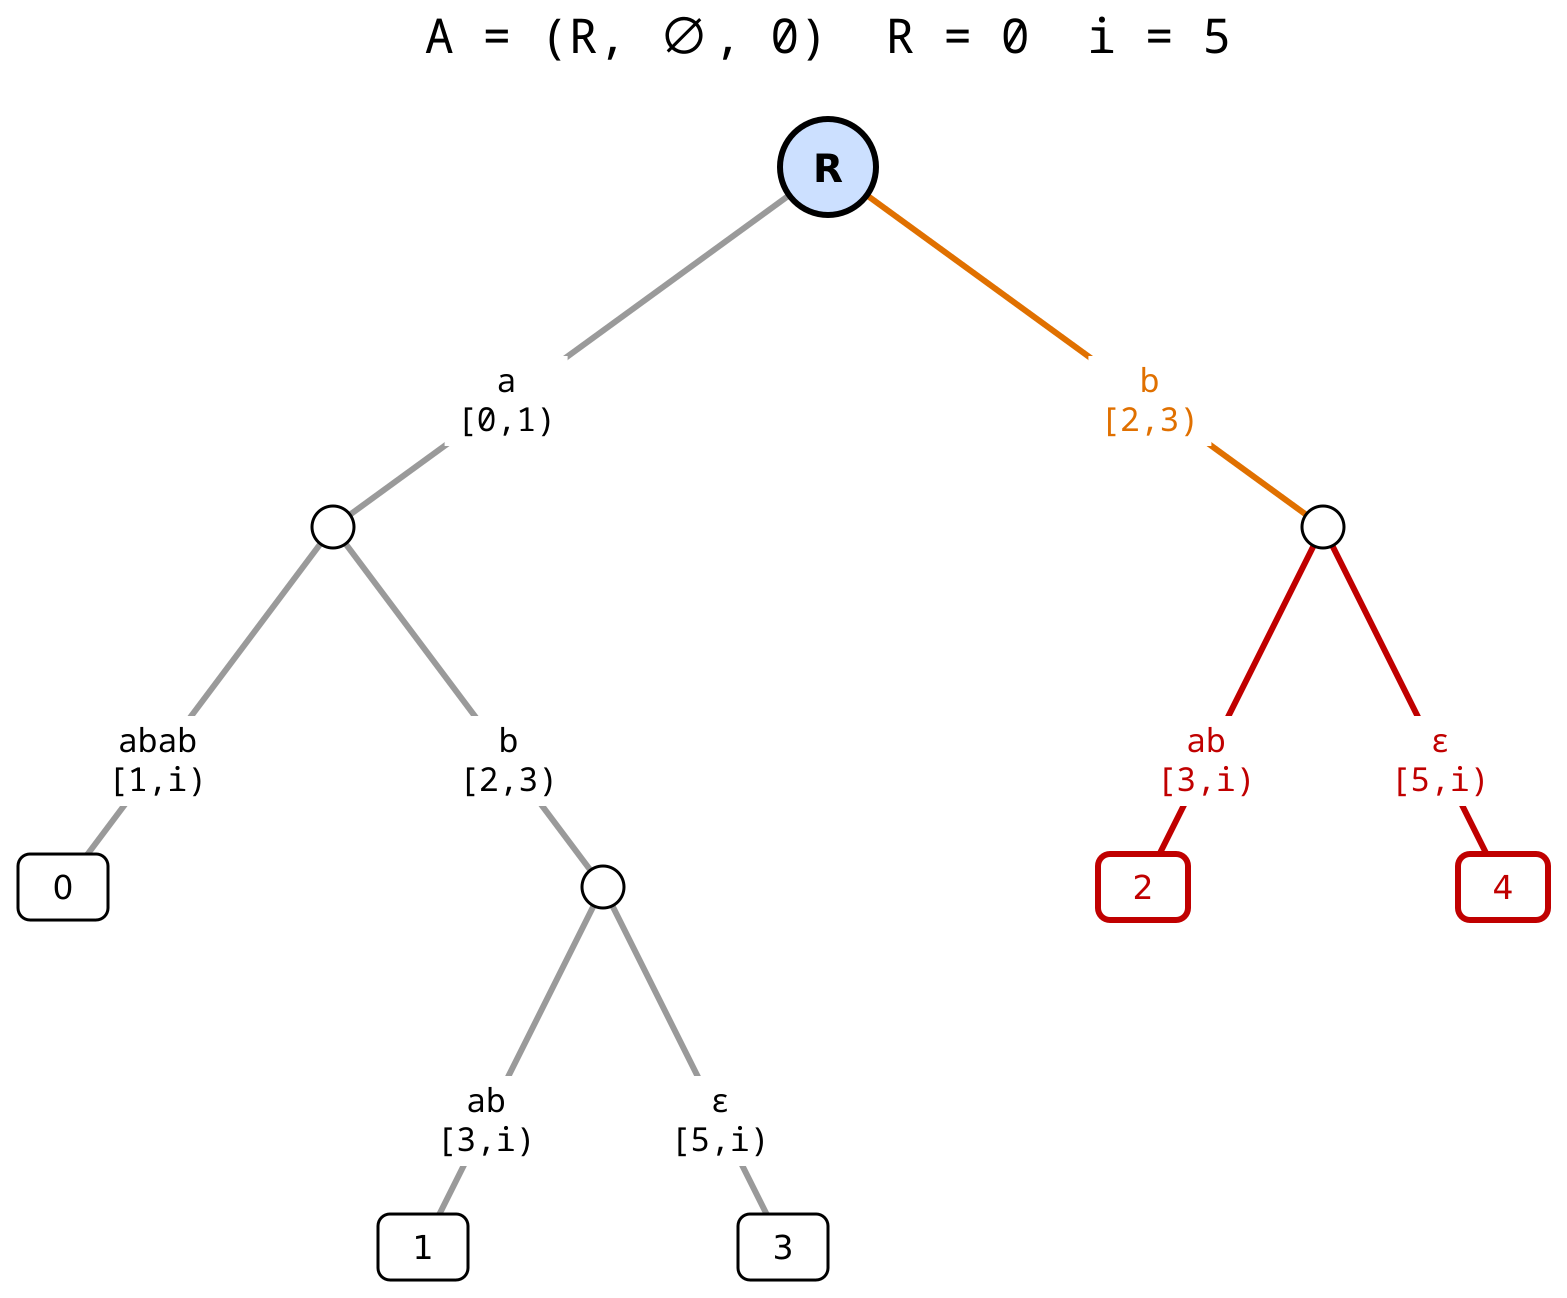
\includegraphics[scale=0.17]{media/Example/step09}
		\caption{The root's leaf \texttt{bab} is split after \texttt{b}.}
		\label{fig:step09}
	\end{figure}
	From the root, $e$ is chosen by $s[\textbf{i} - len] = s[4] =$ 'b', which is the root's leaf $(2, \textbf{i})$, also spelling 'bab'.  Again, $s[2 + len] = s[3] =$ 'a' is not \$, so this edge is split in the same way, inserting the suffix 'b\$'.  \textbf{R} is reduced to 0, so \textbf{i} stays at 5 and $len = 0$.

	\paragraph{11. Add New Node.}\leavevmode
	\begin{figure}[H]
		\centering
		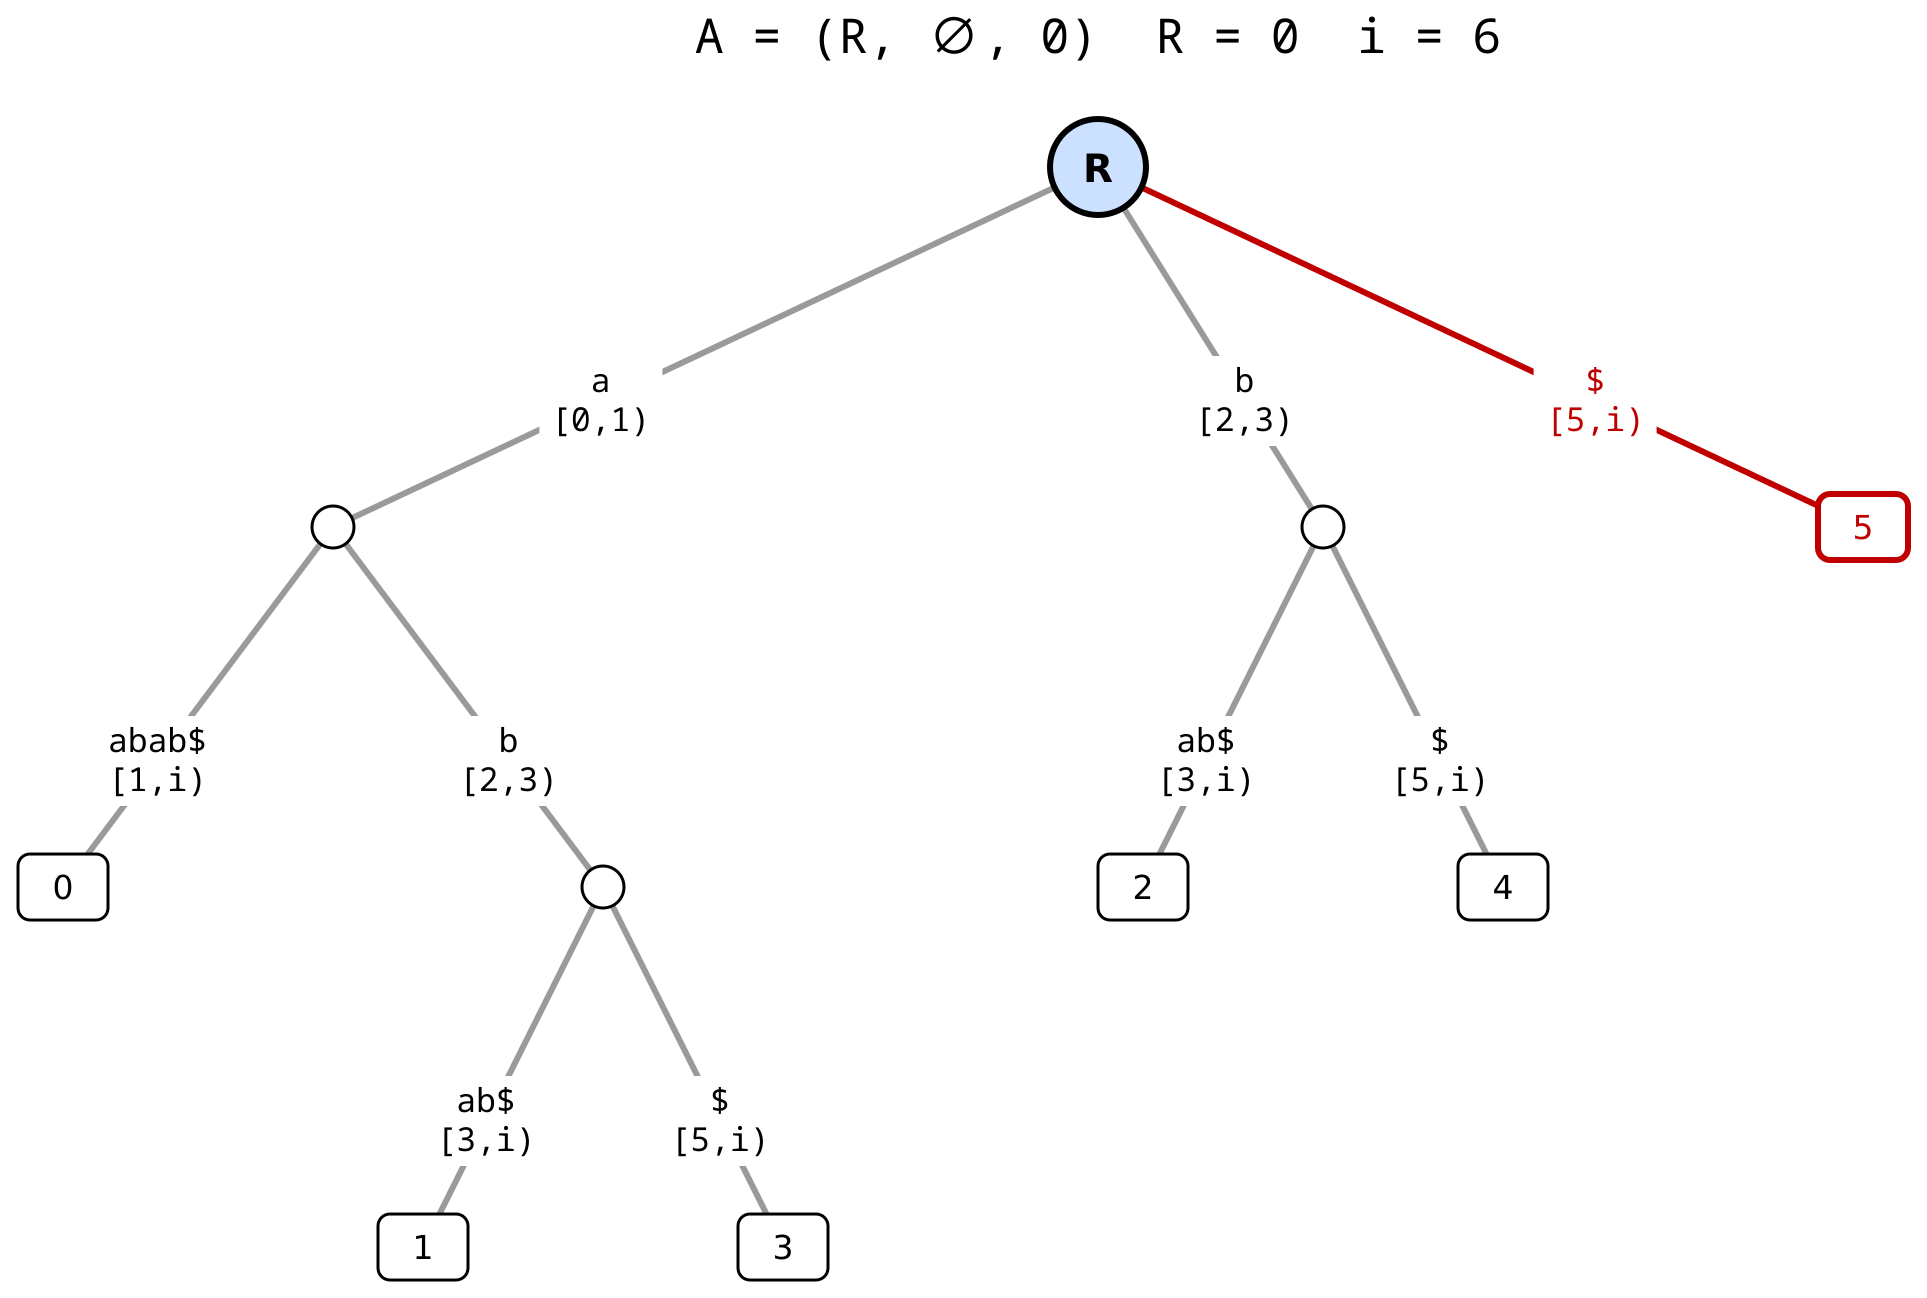
\includegraphics[scale=0.17]{media/Example/step10}
		\caption{The completed suffix tree of \texttt{aabab\$}.}
		\label{fig:step10}
	\end{figure}
	Only the suffix '\$' remains.  The root has no child beginning with \$, so (Rule.2) creates a new node from $(5, \textbf{i})$.  As \textbf{R} = 0, \textbf{i} is increased to 6, which is past the end of 'aabab\$', so the loop ends.  The completed tree has six leaves, one for each suffix of 'aabab\$'.
	
	\subsection{Where Suffix Links Differ}

	\paragraph{Between Steps 4 and 5.}\leavevmode
	\begin{figure}[H]
		\centering
		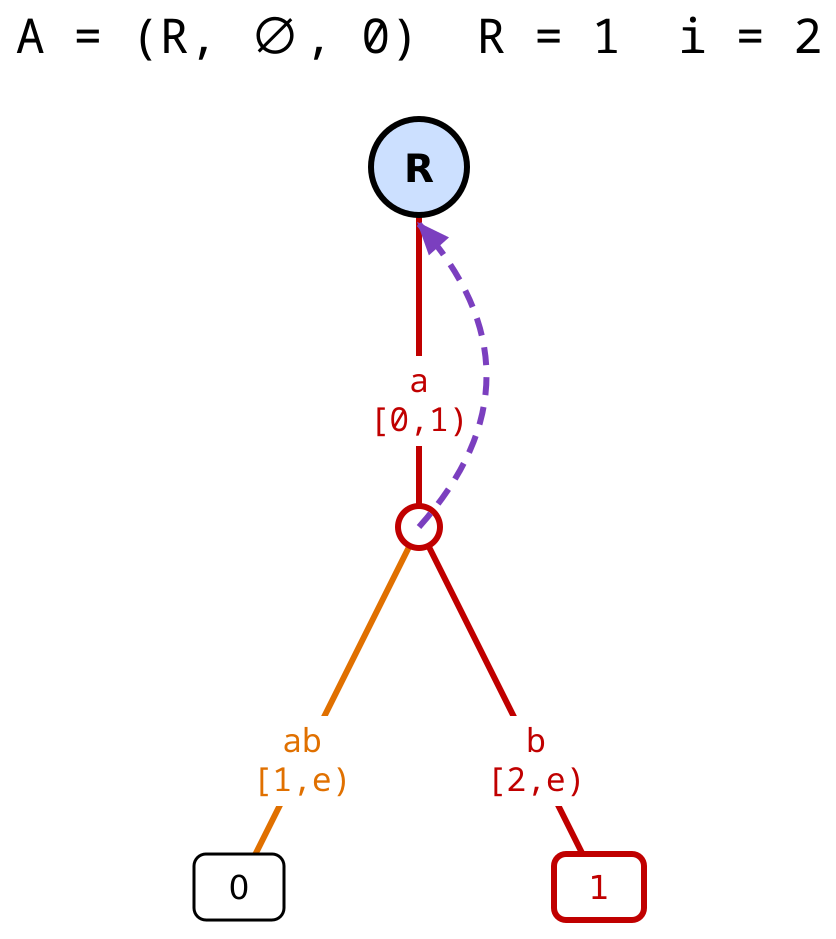
\includegraphics[scale=0.17]{media/SuffixLinks/step03}
		\caption{The new internal node \texttt{a} is given a suffix link to the root.}
		\label{fig:links04}
	\end{figure}
	In the suffix link version, the split at \textbf{i} = 2 inserts a new internal node from $(0, 1)$ above the old leaf, rather than shortening the old node in place, so the old leaf's edge now begins at index 1.  The new internal node spells 'a', and removing its first character leaves the empty string, so its suffix link points to the root.  As $\rho$ is the root, $len$ is reduced by one to 0, rather than being set to \textbf{R}.  \textbf{R} = 1 here, not 0, because this version also counts the current character's suffix, 'b', as pending.
	
	\paragraph{Between Steps 9 and 10.}\leavevmode
	\begin{figure}[H]
		\centering
		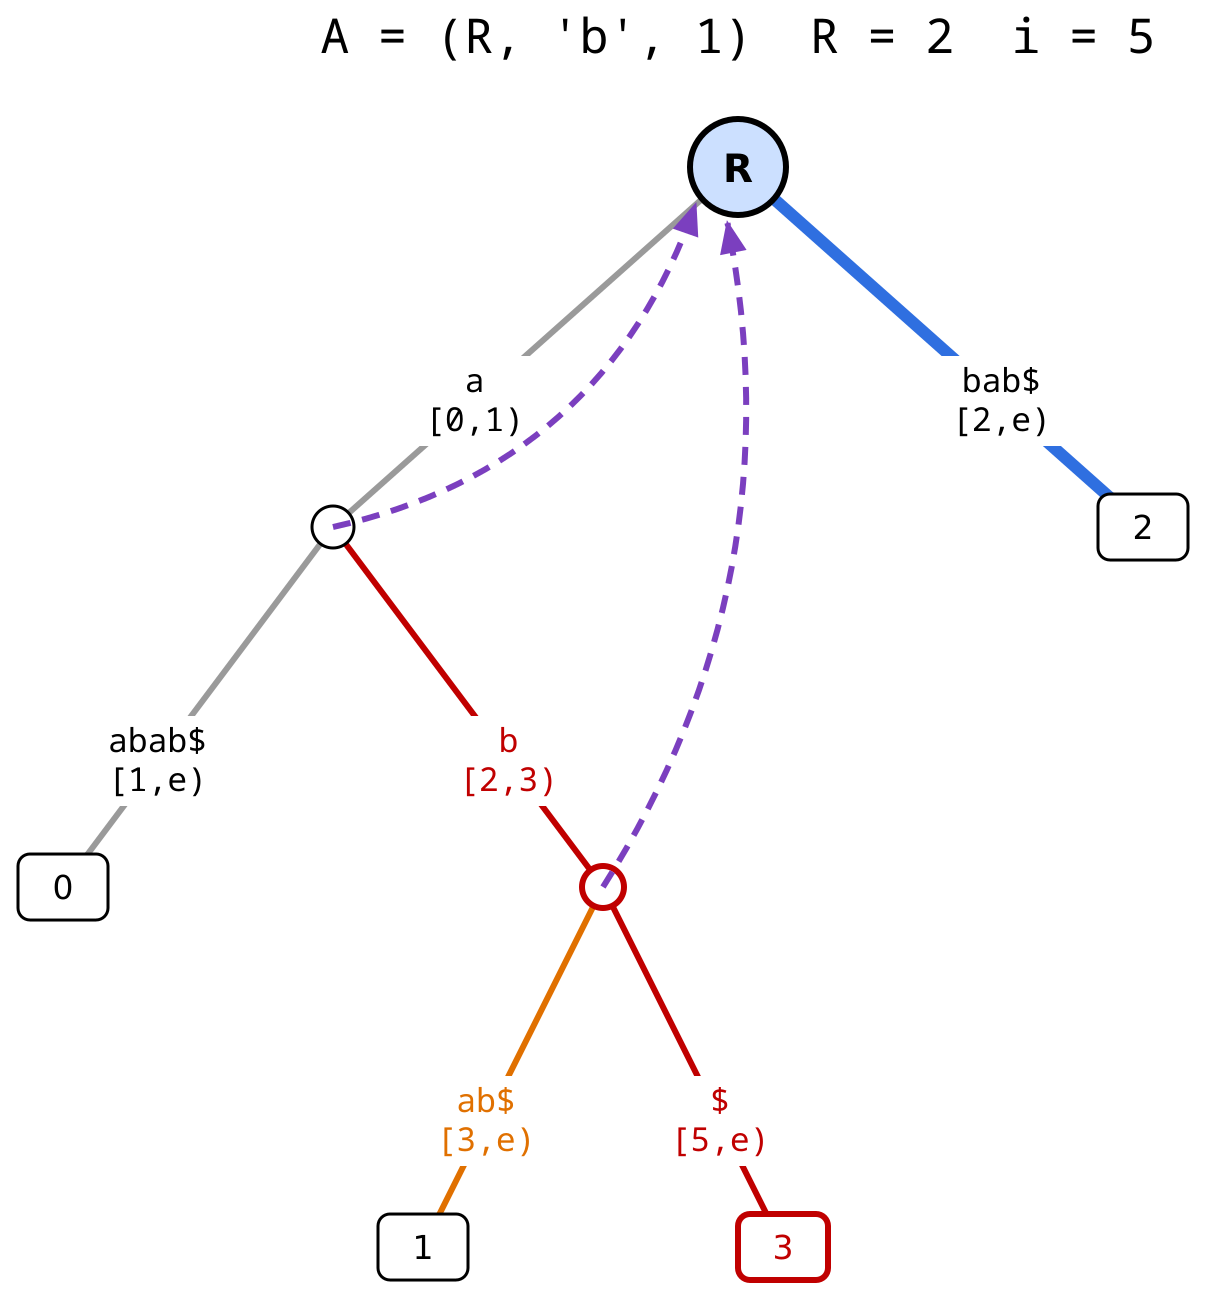
\includegraphics[scale=0.17]{media/SuffixLinks/step08}
		\caption{The active point follows the suffix link of \texttt{a} to the root, instead of resetting.}
		\label{fig:links09}
	\end{figure}
	At \textbf{i} = 5, the leaf below the internal node 'a' is split after 'b', creating the internal node 'ab', which is given a suffix link to the root for now.  In my implementation, the active point then resets to the root with $len$ set to \textbf{R}.  Here, $\rho$ is not the root, so the active point follows the suffix link of 'a' instead, keeping $e$ and $len = 1$.  The link of 'a' points to the root, so both versions reach the same position, but when a link points to another internal node, following it avoids traversing down again from the root.
	
	\paragraph{Between Steps 10 and 11.}\leavevmode
	\begin{figure}[H]
		\centering
		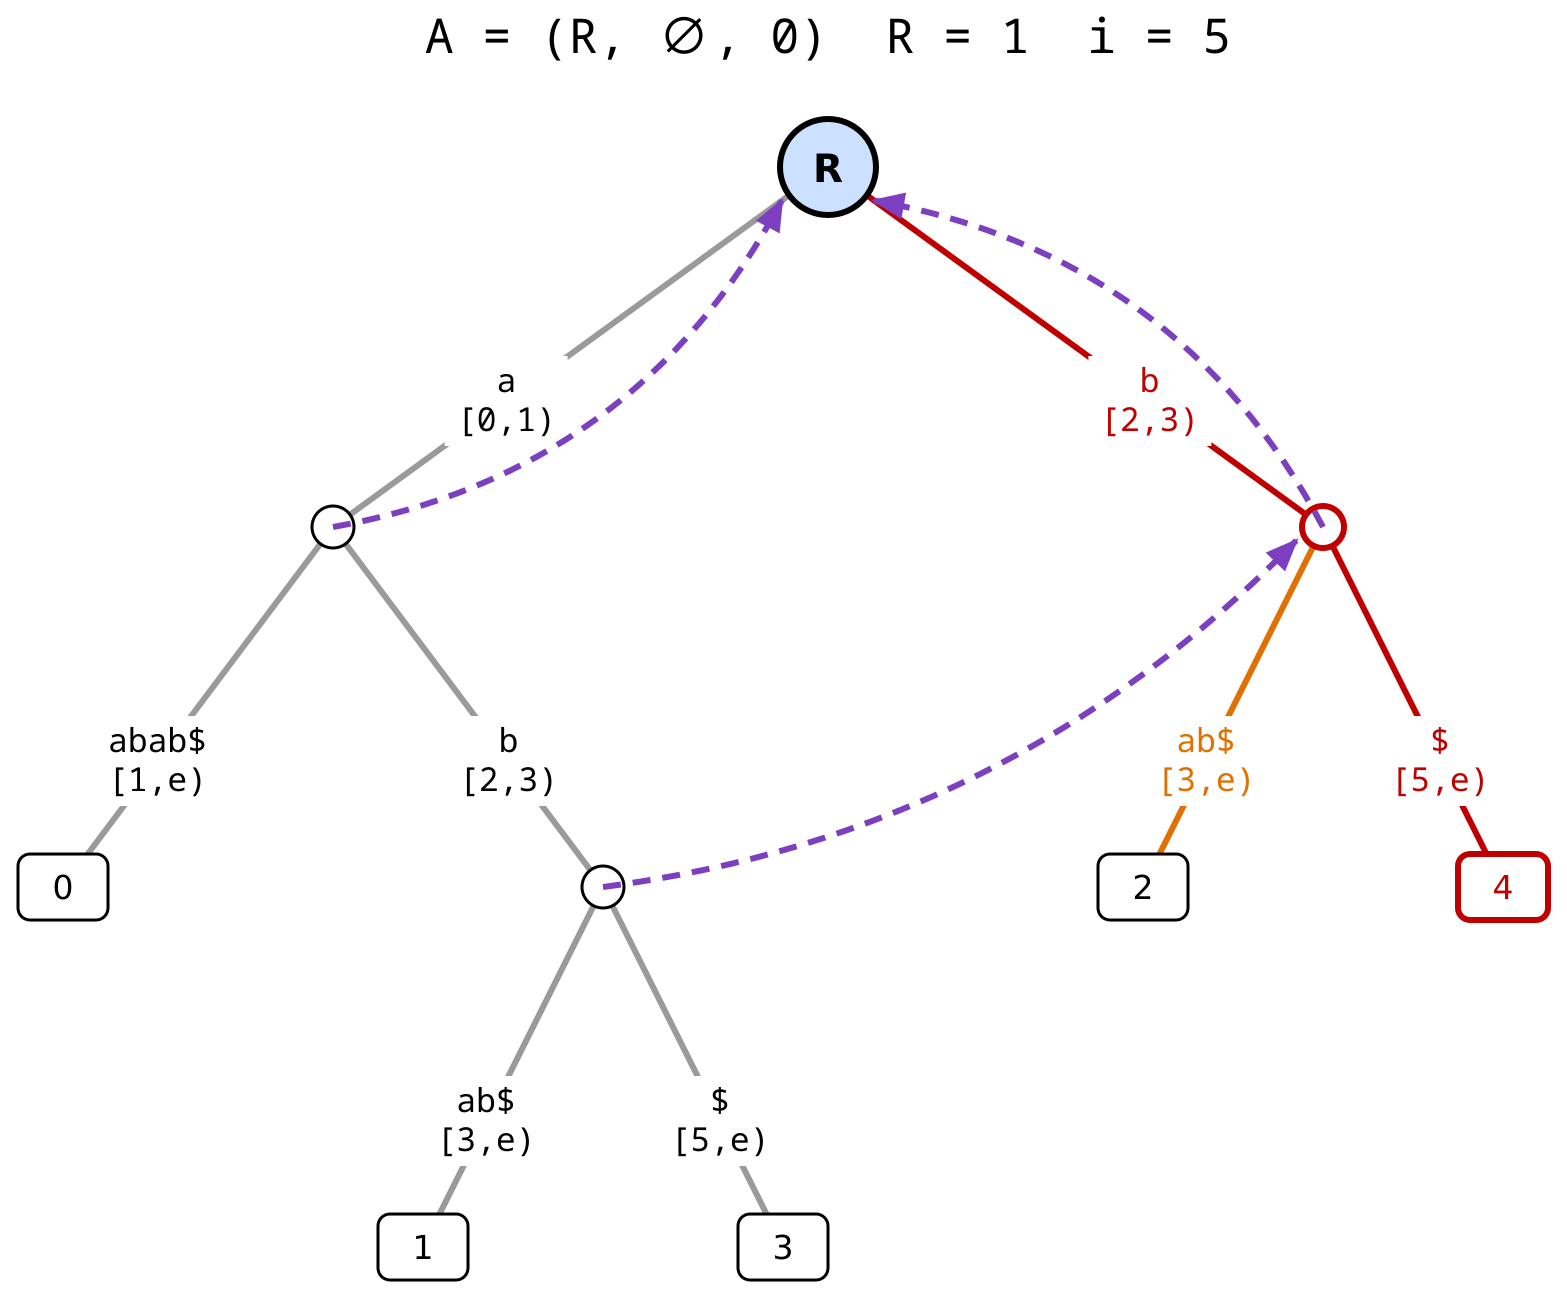
\includegraphics[scale=0.17]{media/SuffixLinks/step09}
		\caption{\texttt{ab} now links to \texttt{b}, and \texttt{b} links to the root.}
		\label{fig:links10}
	\end{figure}
	From the root, the leaf 'bab\$' is split after 'b', creating the internal node 'b'.  As 'ab' was the last internal node created in this phase, its suffix link is set to 'b', since removing the first character of 'ab' leaves 'b'.  The new node 'b' links to the root.  As $\rho$ is the root, $len$ is reduced by one to 0, and the next step adds the \$ leaf as in my implementation.

	\section{The Correctness of  The Naive Ukkonen's Algorithm}
	
	\paragraph{Precondition:}
	Let $\Sigma$ exist as an alphabet such that $\$ \notin \Sigma$, and where $L$ exists that $L \subseteq \Sigma^*$ .  There must be some string s, such that $s \in L$, also represented as $s = s_0, s_1 \dots s_{n - 1}$. 

	\paragraph{Post-condition: (P0.)} 
	Given string $s$, where $\sigma(s)$ constructs a suffix tree of $s$.  It is, then, expected that:
	
	\begin{enumerate}[label=(P0.\arabic*), ref=(P0.\arabic*)]
		\item the root node, $R$, exists such that $\sigma(s) = R$
		\item $R$ contains at least one node for the terminal \$, $\nu_{n}$ and where $\eta_R$ = $\{\nu_0 \dots \nu_n \}$.
		\item where $\alpha(\nu)$ is the inclusive beginning and $\beta(\nu)$ is the exclusive ending of $\nu$, $\forall \nu \in \eta_R, 0 \le \alpha(\nu) \le \beta(\nu) \le n + 2$.
		\item all child nodes of $R$ must have a unique beginning index, $\forall i, j \in \{0\dots n\}, i \ne j: \alpha(\nu_i) \ne \alpha(\nu_j)$.
		\item where $R$ is the root of suffix tree $T_R$, $\forall \nu \in \eta_R, \{\exists T_{\nu} | \nu \ne \nu_n\}$.
		\item it follows, $\forall \nu\prime \in \eta_R, \{\exists T_{\nu\prime} | \nu\prime \ne \nu_{|\eta_{\nu\prime}|}\}$.
		\item any possible sub-string $s[i, j]$ where $0 \le i \le j \le n$, can be searched within $T_R$.
	\end{enumerate}
	
	\subsection{Initialisation}
	
	\paragraph{Post-condition: (P1.)}
	Following initialisation, it is expected that:
	\begin{enumerate}[label=(P1.\arabic*), ref=(P1.\arabic*)]
		\item $R$ exists such that $\alpha(R) = \beta(R) = \bot$.
		\item the active point, $AP$, contains parent node $\rho$, such that $\rho = R$.
		\item there is some global index $i$, such that any node $\nu$ where $\beta(\nu) = i$, then on $i = i + 1$, $\beta(\nu) = i + 1$.  
		\item there is also $i\prime$ where instead $\beta(\nu) = i\prime$ when $i = i + 1$.
	\end{enumerate}
	
	\subsection{The Main Loop}
	\paragraph{Post-condition: (P2)} given the main loop is the entirety of the algorithm outside of initialisation, then (P2) holds the same post-conditions as (P0).
	
	\paragraph{Loop Invariant: (I)}
	\begin{enumerate}[label=(I.\arabic*)]
		\item That $0 \le i \le n + 2$.
		\item $\alpha(R) = \beta(R) = \bot$.
		\item Where $rem$ denotes the remainder, then $0 \le rem \le n$.
		\item Where $len$ denotes the length in AP, then $0 \le len \le n + 1$.
		\item There is $\tau_{(i, rem)}$, a partially constructed suffix tree at operation $(i, rem)$, such that $\rho \in N\tau_{(i, rem)}$.  Allow $N\tau_{(i, rem)}$ to be the set of all nodes in $\tau_{(i, rem)}$.
	\end{enumerate}
	
	\paragraph{Loop Variant:} The loop terminates for the following $(n + 1 - i, rem, len)$.  $n + 1 - i$, .  
	\begin{enumerate}
		\item $n + 1 - i$ allows the loop to access all characters in s, as well as the \$ before reaching $0$
		\item $rem$ exists such that it tracks the number of remaining suffixes yet to be placed into the tree.  All suffixes of $s$ must be placed into the tree, thus $rem$ must be $0$ for the loop to terminate.
		\item $len$ tracks how far into an edge is currently being compared.  Each edge split will reduce the length to $rem$, and so for the loop to terminate $len$ must be $0$.
	\end{enumerate}
	
	\subsection{Searching For a  Node}
	\paragraph{Post-condition: (P3)} Either a node, $\nu$ is found such that $\nu \in N\tau_{(i, rem)}$ (Case 2), or the node doesn't exist (Case 1). All of \textbf{(I)}holds.
	
	\begin{lemma}The only node which ever is searched for any child node, is $\rho$.\end{lemma}
	
	\begin{proof}There is only one occurrence of searching for a child node, on \textbf{line 36}.  The exact node being searched against is $\rho$.\end{proof}
	
	\paragraph{Case 1: no such child exists.}
	\subparagraph{Post-condition (P3.a)} .  
	\begin{enumerate}[label=(P3.a.\arabic*), ref=(P3.a.\arabic*)]
		\item A new node, $\nu$ is created such that $\alpha(\nu) = i\prime - len$.
		\item $\nu \in \eta_{\rho}$.
	\end{enumerate}

	\begin{lemma} Where no node was initially found, the creation of any node $\nu$ at operation $(i, rem)$, must only become a child of $\rho$, $\eta_{\rho} = \eta_{\rho}  \cup \nu$.\end{lemma}
	
	\begin{proof} On \textbf{line 42}, the node $\nu$ is created, where only \textbf{line 45} $\nu$ becomes a child of $\rho$.   The only other occurrence of insertion is on \textbf{lines 97, 98}, where the edge is split.\end{proof}
	
	\begin{lemma}
		Where a node was not found, creating a child node ends the operation.
	\end{lemma}
	\begin{proof}
		On \textbf{line 58}, the clause which allows for the creation of a node skips and moves to either operation $(i + 1, 0)$ or $(i, rem - 1)$.
	\end{proof}
	
	\textit{The loop is re-iterated.} A new node has been created, and (Rule.2) is complete.
		
	\textit{Importance.}  Creating a new node, $\nu$, at $(i, rem)$ allows for the addition of new suffixes of $s$.
	
	\textit{Omission means,} initially on operation (0, 0), when $\rho = R$, then $s[i\prime - len]$ can never create a new node, preventing (P0.2).  All of \textbf{(I)} would hold.
	
	\subparagraph{Case 2: Use an existing node.}
	\subparagraph{Post-condition: (P3.b).} The edge node in $AP$, $e = \forall \nu\prime \in \eta_{\rho}, \{\exists s[\alpha(\nu\prime)] = s[i\prime - len]\}$.

	\begin{lemma}
		Before the edge is not split, there cannot be any two nodes, which their first indices index the same character in $s$ on $\rho$, $\forall \nu\prime \in \eta_{\rho}, \{\exists s[\alpha(\nu\prime)] = s[i\prime - len]\}$.
	\end{lemma}
	
	\begin{proof}
		All edge split logic occurs on \textbf{lines 97, 98}.   
		By \textbf{Lemma 4.1} and \textbf{Lemma 4.2}, a node can only be added if it's not found.  Because the node is found, it cannot be added, and therefore there can never have nodes such that any two beginning indices point to the same character in $s$.  In order for \textbf{(P3)} to hold, then a node must be selected, which already exists, fulfilling \textbf{(P3.b)}.
	\end{proof}
	
	\textit{Importance.} There must be an edge so that either (Rule.2) or (Rule.3) may be applied.  All of \textbf{I} still holds.
	
	\textit{Omission means,} the edge can never be split at an operation.  Therefore, \textbf{(P0.4)} will always fail.

	
	\subsection{Equality of Characters}	
	\subsubsection{Case 1: Length is outside the edge}
	\subparagraph{Post-condition: (P5.a).} 
	\begin{enumerate}[label=(P5.a.\arabic*), ref=(P3.a.\arabic*)]
		\item The value of $e$ moves to $\rho$.
		\item $len < \beta(\rho) - \alpha(\rho)$
		\item $e = \bot$.
	\end{enumerate}
	
	\begin{lemma}
		For any character comparisons, $len < \beta(e) - \alpha(e)$.
	\end{lemma}
	\begin{proof}
		\textbf{Lines 66, 76 and 113} all exist exclusively such that only one can be done in each iteration.  Therefore, whenever $len \ge \beta(e) - \alpha(e)$, the length is updated to fit within a new edge.
	\end{proof}
	\textit{Importance.} There must be a valid character comparison so (Rule.2) or (Rule.3) may be applied.  All of \textbf{I} still holds.

	\textit{Omission means,} any edge $e$ can allow comparisons of characters greater than $\beta(e)$, introducing suffixes which do not exist, and breaking \textbf{(P0.7)}.
	
	\subsubsection{Case 2: Splitting the Edge}
	\subparagraph{Post-condition: (P5.b).} 
	\begin{enumerate}[label=(P5.b.\arabic*), ref=(P3.a.\arabic*)]
		\item $\beta(e) = i\prime - len$.
		\item allow $\tau_{s[i\prime - len], (i, rem)}$ to be the partially constructed suffix tree, where, $e$ exists as the root node.  Then, $|\eta_{\tau_{s[i\prime - len], (i, rem)}}| = 2$.
		\item The first node $\nu_0$ in $\eta_{\tau_{s[i\prime - len], (i, rem)}}$ exists such that $\alpha(\nu_0) = i\prime$ and $\beta(\nu_0) = i$.
		\item The second node $\nu_1$ also exists, such that $\alpha(\nu_1) = i\prime - len$, and $\beta(\nu_1) = i$.
	\end{enumerate}
	
	\paragraph{Creating New Nodes}
	\begin{enumerate}[label=(P5.b.\arabic*), ref=(P3.a.\arabic*)]
		\item There exist two nodes, $\nu_0$ and $\nu_1$ without any incoming edges or children.
		\item $\nu_0$ exists such that $\alpha(\nu_0) = i\prime$ and $\beta(\nu_0) = i$.
		\item $\nu_1$ also exists, such that $\alpha(\nu_1) = i\prime - len$, and $\beta(\nu_1) = i$.
	\end{enumerate}
	
	\begin{lemma}
		The first new node, $\nu_0$, exists such that $\alpha(\nu_0) = i\prime$ and $\beta(\nu_0) = i$.
	\end{lemma}
	\begin{proof}
		The only point where a first node is created is on \textbf{line 97}, which uses indices from \textbf{line 79}.  The indices are $(i\prime, i)$.
	\end{proof}
	
	\begin{lemma}
		The second new node, $\nu_1$, exists such that $\alpha(\nu_1) = i\prime - len$ and $\beta(\nu_1) = i$.
	\end{lemma}
	\begin{proof}
		The only point where a second node is created is on \textbf{line 88}, which uses indices from \textbf{line 82}.  The indices are $(i\prime - len, i)$.
	\end{proof}
	
	\textit{importance.}  A split cannot occur without two new nodes.
	\textit{Omission means,} the split simply cannot occur, and the tree becomes an implicit suffix tree.
		
	\paragraph{Transferring of Child Nodes}	
	\subparagraph{Post-condition: (P5.c).}
	\begin{enumerate}[label=(P5.c.\arabic*), ref=(P3.a.\arabic*)]
		\item $\nu_1$ contains old children
		\item $e$ contains no children
	\end{enumerate}

	\begin{lemma}
		When an edge is split, all of children in $e$ must be moved to $\nu_1$.
	\end{lemma}
	\begin{proof}
		The only occurrence of any children being moved is on \textbf{line 91}.  This explicitly sets $\nu_1$ as to retrieve the children of $e$.  Then, on \textbf{line 94}, all of the children which existed in $e$ are cleared in memory.
	\end{proof}
	
	\textit{importance.} In order for an edge to be split, the children of $e$ must be moved to $\nu_1$.
	\textit{Omission means, } that $e$ will allow for the searching of characters which do not occur after it, thus breaking \textbf{(P0.7)}.
	
	\paragraph{Adding the New Nodes}
	\begin{enumerate}[label=(P5.d.\arabic*), ref=(P3.a.\arabic*)]
		\item $|\tau_{s[i\prime - len], (i, rem)}| = 2$ 
	\end{enumerate}
	
	\begin{lemma}
		Only two nodes can be created from a split such that they join e.
	\end{lemma}
	
	\textit{Importance.}  The edge is split, so the nodes must be added.
	\textit{Omission means} There is no way to add suffixes which share a common beginning unless its the largest suffix.
	
	\subsubsection{Case 3: Skipping Operation}
	\paragraph{Post-condition: (P6)} Same as (P0).  Loop invariant holds.
	
	\begin{lemma}
		Characters can be equal.
	\end{lemma}
	
	\textit{Importance.} When two indices are equal this does not mean it should split the edge.
	\textit{Omission means}  New suffixes will be added which are not part of the string.
	
	\subsection{Conclusion}
	The algorithm meets all the necessary lemmas such that the root node will return the root of a constructed suffix tree without suffix links.  As demonstrated, all of Ukkonen's extension rules are complete.
		
	\section{Running the Algorithm}
	The algorithm itself exists solely and entirely as a raw implementation.  There is no other piece of code which uses it, outside of the custom test runner, which was built to run JSON test cases against the algorithm.
	
	\subsection{Test Run Results}
	\subparagraph{Considerations: }
	\begin{enumerate}
		\item These were run locally on a PC once, all sequentially in the same process.
		\item Running time is calculated using the \textit{<chrono>} library in \textit{C++}, with \textit{time after execution - time before execution}.
		\item Whilst inflated, it proves in the very least that the running time is at least as fast as the provided values.
	\end{enumerate}
	
	\subparagraph{Observations: }
	\begin{enumerate}
		\item The empty string, $\varepsilon$ has the shortest running time.
		\item The longest string 'abcdefabxybcdmnabcdex' has the longest running time.
		\item There is some correlation such that the larger the word size, the longer the running time.
		\item There is a lack of correlation between running time and alphabet size.
	\end{enumerate}
	
	\begin{table}[ht]
	\centering
	\caption{Suffix tree construction results.}
	\label{tab:results}
	\scriptsize
	\setlength{\tabcolsep}{3.5pt}
	\renewcommand{\arraystretch}{1.25}
	\setlength{\aboverulesep}{0pt}
	\setlength{\belowrulesep}{0pt}
	\rowcolors{2}{gray!12}{white}
	\begin{tabular}{l c r r r r c}
		\toprule
		\rowcolor{blue!15}
		Word & Passed & Word Size & Alphabet Size & Total Nodes & Time (ms) & $<$ \qty{30}{\micro\second} \\
		\midrule
		$\varepsilon$                    & \textcolor{green!50!black}{Yes} &  0 & 0 &  2 & 0.0009 & \textcolor{green!50!black}{Yes} \\
		\texttt{a}                       & \textcolor{green!50!black}{Yes} &  1 & 1 &  3 & 0.0014 & \textcolor{green!50!black}{Yes} \\
		\texttt{ab}                      & \textcolor{green!50!black}{Yes} &  2 & 2 &  4 & 0.0021 & \textcolor{green!50!black}{Yes} \\
		\texttt{aa}                      & \textcolor{green!50!black}{Yes} &  2 & 1 &  5 & 0.0032 & \textcolor{green!50!black}{Yes} \\
		\texttt{abc}                     & \textcolor{green!50!black}{Yes} &  3 & 3 &  5 & 0.0030 & \textcolor{green!50!black}{Yes} \\
		\texttt{aab}                     & \textcolor{green!50!black}{Yes} &  3 & 2 &  6 & 0.0040 & \textcolor{green!50!black}{Yes} \\
		\texttt{aba}                     & \textcolor{green!50!black}{Yes} &  3 & 2 &  6 & 0.0041 & \textcolor{green!50!black}{Yes} \\
		\texttt{aaa}                     & \textcolor{green!50!black}{Yes} &  3 & 1 &  7 & 0.0050 & \textcolor{green!50!black}{Yes} \\
		\texttt{aaab}                    & \textcolor{green!50!black}{Yes} &  4 & 2 &  8 & 0.0056 & \textcolor{green!50!black}{Yes} \\
		\texttt{abab}                    & \textcolor{green!50!black}{Yes} &  4 & 2 &  8 & 0.0055 & \textcolor{green!50!black}{Yes} \\
		\texttt{baaa}                    & \textcolor{green!50!black}{Yes} &  4 & 2 &  8 & 0.0063 & \textcolor{green!50!black}{Yes} \\
		\texttt{aaaa}                    & \textcolor{green!50!black}{Yes} &  4 & 1 &  9 & 0.0065 & \textcolor{green!50!black}{Yes} \\
		\texttt{xabxac}                  & \textcolor{green!50!black}{Yes} &  6 & 4 & 10 & 0.0067 & \textcolor{green!50!black}{Yes} \\
		\texttt{abcabc}                  & \textcolor{green!50!black}{Yes} &  6 & 3 & 11 & 0.0080 & \textcolor{green!50!black}{Yes} \\
		\texttt{banana}                  & \textcolor{green!50!black}{Yes} &  6 & 3 & 11 & 0.0138 & \textcolor{green!50!black}{Yes} \\
		\texttt{abacaba}                 & \textcolor{green!50!black}{Yes} &  7 & 3 & 12 & 0.0089 & \textcolor{green!50!black}{Yes} \\
		\texttt{cdddcdc}                 & \textcolor{green!50!black}{Yes} &  7 & 2 & 14 & 0.0109 & \textcolor{green!50!black}{Yes} \\
		\texttt{xyzxyaxyz}               & \textcolor{green!50!black}{Yes} &  9 & 4 & 16 & 0.0123 & \textcolor{green!50!black}{Yes} \\
		\texttt{abcabcabc}               & \textcolor{green!50!black}{Yes} &  9 & 3 & 17 & 0.0130 & \textcolor{green!50!black}{Yes} \\
		\texttt{abcabxabcd}              & \textcolor{green!50!black}{Yes} & 10 & 5 & 17 & 0.0125 & \textcolor{green!50!black}{Yes} \\
		\texttt{mississippi}             & \textcolor{green!50!black}{Yes} & 11 & 4 & 19 & 0.0148 & \textcolor{green!50!black}{Yes} \\
		\texttt{dedododeeodo}            & \textcolor{green!50!black}{Yes} & 12 & 3 & 22 & 0.0180 & \textcolor{green!50!black}{Yes} \\
		\texttt{abaababaabaab}           & \textcolor{green!50!black}{Yes} & 13 & 2 & 26 & 0.0245 & \textcolor{green!50!black}{Yes} \\
		\texttt{abcdefabxybcdmnabcdex}   & \textcolor{green!50!black}{Yes} & 21 & 10 & 34 & 0.0267 & \textcolor{green!50!black}{Yes} \\
		\bottomrule
	\end{tabular}
	\end{table}
	
	\clearpage
	\section{Use of Generative AI}
	\paragraph{Models Used:} Claude Opus 5.5, via Claude Code (Anthropic)
	\paragraph{Date of Usage:} 20/09/26 to 02/10/26
	
	\begin{table}[H]
		\centering
		\caption{Use of generative AI in this paper.}
		\label{tab:ai-use}
		\scriptsize
		\setlength{\tabcolsep}{3.5pt}
		\renewcommand{\arraystretch}{1.25}
		\setlength{\aboverulesep}{0pt}
		\setlength{\belowrulesep}{0pt}
		\rowcolors{2}{gray!12}{white}
		\begin{tabular}{
				>{\raggedright\arraybackslash}p{0.14\linewidth}
				>{\raggedright\arraybackslash}p{0.26\linewidth}
				>{\raggedright\arraybackslash}p{0.30\linewidth}
				>{\raggedright\arraybackslash}p{0.22\linewidth}}
			\toprule
			\rowcolor{blue!15}
			Area & What I Did & What AI Did & Purpose \\
			\midrule
			Formatting & Wrote the document structure and content. & Set up the code listings, figure placement and table styling. & The document compiles cleanly and reads well. \\
			Diagrams & Chose \texttt{aabab} as the example and specified the layout. & Generated the step images and the suffix link images. Red marks new nodes, orange a shortened edge, the shaded node the active parent and the thick blue edge the active edge. & Each step of the walk-through is shown visually. \\
			Step 1 (Fig.~\ref{fig:step00}) & Wrote the step description. & Generated the image of the root alone, with $A = (R, \emptyset, 0)$, $R = 0$ and $i = 0$ above it. & Shows the state after initialisation. \\
			Step 2 (Fig.~\ref{fig:step01}) & Wrote the step description. & Generated the image of the new leaf for \texttt{a} under the root, drawn in red, with $i$ advanced to 1. & Shows a new node being created. \\
			Step 3 (Fig.~\ref{fig:step02}) & Wrote the step description. & Generated the image of rule 3, with the active edge \texttt{a} in blue, $A = (R, \texttt{a}, 1)$ and $R = 1$. & Shows a suffix being deferred. \\
			Step 4 (Fig.~\ref{fig:step03}) & Wrote the step description. & Generated the image of the leaf \texttt{aa} split after \texttt{a}, with the shortened edge in orange and the new internal node and leaf in red. & Shows an edge being split. \\
			Step 5 (Fig.~\ref{fig:step04}) & --- & Generated the image of the new leaf for \texttt{b} under the root, with $i$ advanced to 3. & Shows a new node added at the root. \\
			Step 6 (Fig.~\ref{fig:step05}) & --- & Generated the image of rule 3 on the internal edge \texttt{a}, with $R = 1$ and a length of 1. & Shows a deferral along an internal edge. \\
			Step 7 (Fig.~\ref{fig:step06}) & --- & Generated the image of the walk-down, with the internal node \texttt{a} shaded as the new parent and a length of 0. & Shows edge traversal. \\
			Step 8 (Fig.~\ref{fig:step07}) & --- & Generated the image of rule 3 below the internal node, with $A = (\texttt{a}, \texttt{b}, 1)$ and $R = 2$. & Shows two suffixes pending. \\
			Step 9 (Fig.~\ref{fig:step08}) & --- & Generated the image of the leaf \texttt{bab} below the internal node split after \texttt{b}, with $A = (R, \emptyset, 1)$ and $R = 1$. & Shows a split below an internal node. \\
			Step 10 (Fig.~\ref{fig:step09}) & --- & Generated the image of the root's leaf \texttt{bab} split after \texttt{b}, with $R = 0$. & Shows the next pending suffix inserted. \\
			Step 11 (Fig.~\ref{fig:step10}) & --- & Generated the image of the new \$ leaf and the completed tree, with six leaves numbered 0 to 5. & Shows the final suffix tree. \\
			Step Explanations & Wrote the explanations for steps 1 to 4. & Wrote the explanations for steps 5 to 11, following my notation. & Every step of the walk-through is explained. \\
			Suffix Link Explanations & Chose the format for where the two versions differ. & Wrote the explanations for the three suffix link figures. & The differences from suffix links are explained. \\
			Captions and Headings & Named the steps. & Wrote the figure captions and renamed some step headings. & Each figure matches its step. \\
			Results Table & Built the test runner and its timing. & Filled the table from a test run and added the pass and timing columns. & The results are reported accurately. \\
			Introduction & Wrote the introduction. & Reviewed it for errors and suggested citations. & The background is accurate. \\
			Invariants & Worked out the invariants on paper. & Clarified the concepts with examples and checked my reasoning. & The correctness argument is sound. \\
			Loop Variant & Wrote the loop variant. & Reviewed it and tested it on an instrumented copy of the code, then explained what was missing from the argument. & The termination argument can be checked. \\
			Complexity Analysis & Wrote the complexity analysis, then removed it. & Reviewed it, counted loop iterations on test strings, and changed the running time claim in the abstract. & The abstract matches the paper. \\
			References & Found the Duke notes and chose the page and line numbers. & Formatted the citations and the bibliography entry in IEEE style. & Sources are cited correctly. \\
			Final Review & Asked for a review before submission. & Listed missing explanations, incorrect notation, sections to split and missing parts. & Remaining issues are known. \\
			Proofreading & Approved the list of quick fixes. & Fixed spelling and notation errors, removed an empty subsection, and labelled each proof with its lemma number. & The document reads correctly. \\
			\bottomrule
		\end{tabular}
	\end{table}
	
	\begin{thebibliography}{9}
		\addcontentsline{toc}{section}{References}
		\bibitem{ukkonen1995} E.~Ukkonen, ``On-line construction of suffix trees,'' \emph{Algorithmica}, vol.~14, no.~3, pp.~249--260, Sep.\ 1995, doi: 10.1007/BF01206331.
		\bibitem{weiner1973} P.~Weiner, ``Linear pattern matching algorithms,'' in \emph{Proc. 14th Annu. Symp. Switching and Automata Theory (SWAT 1973)}, Oct.\ 1973, pp.~1--11, doi: 10.1109/SWAT.1973.13.
		\bibitem{gusfield1997} D.~Gusfield, \emph{Algorithms on Strings, Trees and Sequences: Computer Science and Computational Biology}. Cambridge, U.K.: Cambridge Univ.\ Press, 1997, doi: 10.1017/CBO9780511574931.
		\bibitem{gomez} P.~G\'{o}mez, ``Suffix trees and its construction,'' ch.~5, pp.~49--71, course notes, COMPSCI 260, Duke Univ., Durham, NC, USA, Fall 2014. [Online]. Available: \url{https://courses.cs.duke.edu/fall14/compsci260/resources/suffix.trees.in.detail.pdf} (accessed Oct.\ 2, 2026).
	\end{thebibliography}
\end{document}